% No specific requirements
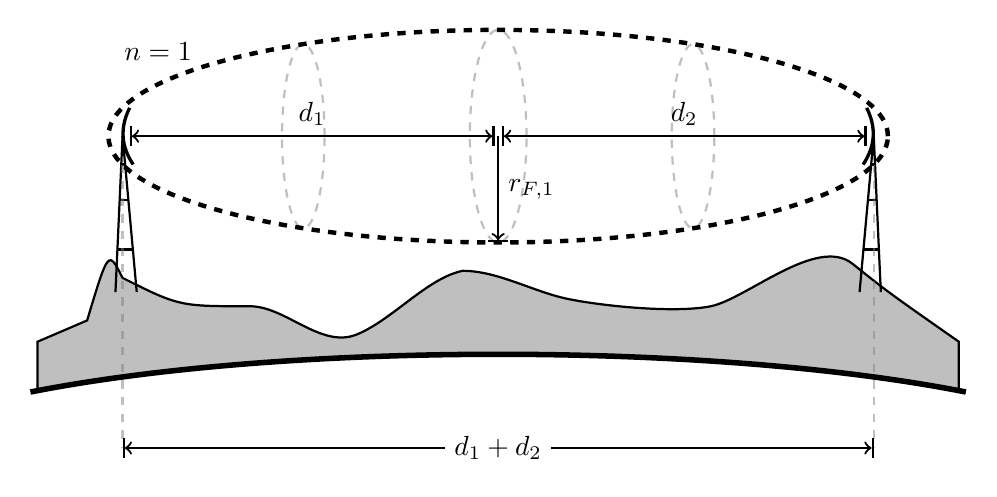
\begin{tikzpicture}[scale=0.9]
  % Earth's Irregular Terrain
  \draw[fill=black,fill opacity =0.25, draw=black, thick]
  (-6.5, 0.5)
  -- (-5.8, 0.8)
  .. controls (-5.5, 1.8) .. (-5.3, 1.4)  % Left peak near tower
  .. controls (-4.5, 1.0) .. (-3.5, 1.0)
  .. controls (-3.0, 1.0) and (-2.5, 0.4) .. (-2.0, 0.6)
  .. controls (-1.5, 0.8) and (-1.0, 1.4) .. (-0.5, 1.5)
  .. controls (0.0, 1.5) and (0.5, 1.2) .. (1.0, 1.1)     % Middle terrain under P
  .. controls (1.5, 1.0) and (2.5, 0.9) .. (3.0, 1.0)
  .. controls (3.5, 1.1) and (4.5, 2.0) .. (5.0, 1.6)     % Right peak near tower
  .. controls (5.5, 1.2) .. (6.5, 0.5)
  -- (6.5, -0.2)
  .. controls (3.0, 0.5) and (-3.0, 0.5) .. (-6.5, -0.2)  % Earth curvature bottom edge
  -- cycle;

  % Thick Blue Earth Curve Line
  \draw[line width=2pt]
  (-6.6, -0.21) .. controls (-3.0, 0.5) and (3.0, 0.5) .. (6.6, -0.21);

  % Antennas (Towers and Focal Dishes)

  % Left Antenna Tower
  \draw[thick] (-5.4, 1.2) -- (-5.3, 3.4) -- (-5.1, 1.2);
  \draw[thick] (-5.37, 1.8) -- (-5.15, 1.8);
  \draw[thick] (-5.34, 2.5) -- (-5.21, 2.5);
  \draw[thick] (-5.31, 3.0) -- (-5.26, 3.0);
  \draw[very thick] (-5.15, 3.0) to[bend left=30] (-5.2, 3.8);

  % Right Antenna Tower
  \draw[thick] (5.1, 1.2) -- (5.3, 3.4) -- (5.4, 1.2);
  \draw[thick] (5.15, 1.8) -- (5.37, 1.8);
  \draw[thick] (5.21, 2.5) -- (5.34, 2.5);
  \draw[thick] (5.26, 3.0) -- (5.31, 3.0);
  \draw[very thick] (5.15, 3.0) to[bend right=30] (5.2, 3.8);

  % Fresnel Zone (Ellipsoid)

  % Inner 3D Gray Rings
  \draw[gray!50!white, dashed,thick] (-2.75, 3.4) ellipse (0.3 and 1.299);
  \draw[gray!50!white, dashed,thick] (0, 3.4) ellipse (0.4 and 1.5);
  \draw[gray!50!white, dashed,thick] (2.75, 3.4) ellipse (0.3 and 1.299);

  % Main Outer Solid Boundary
  \draw[ultra thick,dashed] (0, 3.4) ellipse (5.5 and 1.5);

  % Lines, Arrows, and Labels

  % Distance Labels
  \draw[|<->|, thick] (-5.2, 3.4) -- (-0.05, 3.4) node[midway, above, text=black] {$d_1$};
  \draw[|<->|, thick] (0.05, 3.4) -- (5.2, 3.4) node[midway, above, text=black] {$d_2$};
  \draw[->|,thick] (0, 3.4) -- (0, 1.9) node[midway, right, text=black] {$r_{F,1}$};

  % Fresnel Zone Order Label
  \node at (-4.8, 4.6) {$n = 1$};

  % Distance Vertical Indicator Lines
  \draw[thick,gray,dashed,opacity=0.5] (-5.3, 3.0) -- (-5.3, -1.0);
  \draw[thick,gray,dashed,opacity=0.5] (5.3, 3.0) -- (5.3, -1.0);
  \draw[|<->|,thick] (-5.3, -1.0) -- (5.3, -1.0) node[midway, fill=white] {$d_1+d_2$};

\end{tikzpicture}
